\documentclass[10pt,a4paper,onecolumn]{article}

\usepackage[utf8]{inputenx}
\usepackage[T1]{fontenc}
\usepackage{lmodern}
\usepackage{listings}
\usepackage{textcomp}
\usepackage[english,italian]{babel}
\usepackage{amsmath}
\usepackage{booktabs}
\usepackage{graphicx}
\usepackage[font=small,labelfont=bf,labelsep=period,tableposition=top]{caption}
\usepackage{tabularx}
\usepackage{multirow}
\usepackage{booktabs}
\usepackage{longtable}
\usepackage{fancyhdr}
\usepackage{lastpage}    
\usepackage{color}

\fancyhead{}
\renewcommand{\headrulewidth}{1pt}

\fancyhead[RE,RO]{
\begin{picture}(-135,0)
	%TODO \put(-482,-14){\includegraphics[width=0.26\textwidth]{logoHead.png}} non sono molto bravo con gli strumenti grafici... qualcuno può creare un mini logo da collocare in questa posizione... l'idea è fare la scritta "Progetto di TecWeb... magari a destra di un simbolo che possa rappresentare internet... come... booo.. un mondo con un a rete attorno.... oppure un agglomerato dei loghi di browser come quella che ho scaricato!
	\put(-475,0){\sffamily\large\leftmark}
\end{picture}
}

\cfoot{}

\fancyfoot[RO,LE]{\sffamily Pag.~\thepage{} di \pageref{LastPage}} 
\fancyfoot[RE,LO]{Il mondo di Babe}

\renewcommand{\footrulewidth}{.2pt}
\pagestyle{fancy}

\renewcommand{\sectionmark}[1]{\markboth{#1}{#1}} 

% **************************************************
% Cross-references e collegamenti ipertestuali
% **************************************************
\usepackage[hidelinks]{hyperref}
\hypersetup{%
  colorlinks=false, linktocpage=false, pdfborder={0,0,0}, pdfstartpage=1, pdfstartview=FitV,%
  urlcolor=Cyan, linkcolor=Cyan, citecolor=Black, %pagecolor=Black,
  pdfcreator={pdflatex}, pdfproducer={pdflatex with hyperref package}%
}

\definecolor{dkgreen}{rgb}{0,0.6,0}
\definecolor{gray}{rgb}{0.5,0.5,0.5}
\definecolor{mauve}{rgb}{0.58,0,0.82}
 
\lstset{ %
  language=java,                % the language of the code
  basicstyle=\footnotesize,           % the size of the fonts that are used for the code
  numbers=left,                   % where to put the line-numbers
  numberstyle=\tiny\color{gray},  % the style that is used for the line-numbers
  stepnumber=2,                   % the step between two line-numbers. If it's 1, each line 
                                  % will be numbered
  numbersep=5pt,                  % how far the line-numbers are from the code
  backgroundcolor=\color{white},      % choose the background color. You must add \usepackage{color}
  showspaces=false,               % show spaces adding particular underscores
  showstringspaces=false,         % underline spaces within strings
  showtabs=false,                 % show tabs within strings adding particular underscores
  frame=single,                   % adds a frame around the code
  rulecolor=\color{black},        % if not set, the frame-color may be changed on line-breaks within not-black text (e.g. comments (green here))
  tabsize=2,                      % sets default tabsize to 2 spaces
  captionpos=b,                   % sets the caption-position to bottom
  breaklines=true,                % sets automatic line breaking
  breakatwhitespace=false,        % sets if automatic breaks should only happen at whitespace
  title=\lstname,                   % show the filename of files included with \lstinputlisting;
                                  % also try caption instead of title
  keywordstyle=\color{blue},          % keyword style
  commentstyle=\color{dkgreen},       % comment style
  stringstyle=\color{mauve},         % string literal style
  escapeinside={\%*}{*)},            % if you want to add LaTeX within your code
  morekeywords={*,...},              % if you want to add more keywords to the set
  deletekeywords={...}              % if you want to delete keywords from the given language
}

% **************************************************
% Macro
% **************************************************
\newcommand{\sitepage}[1]{\textsf{#1}}
\newcommand{\inglese}[1]{\foreignlanguage{english}{\itshape{}#1}}

\begin{document}
%----------------------------------------------------------
\begin{titlepage}

\begin{center}
% Upper part of the page
 
\textsc{\Large}\\[5cm]

\includegraphics[width=0.4\textwidth]{Logo.png}\\[0.3cm]  
\noindent\rule{\textwidth}{0.4pt} \\[0.3cm]
\textsc{\Huge Progetto di}\\[0.25cm]
\textsc{\Huge Tecnologie Web}\\[0.3cm]
\textsc{\Large Sito ``Il mondo di Babe''}
\noindent\rule{\textwidth}{0.4pt}\\[0.5cm]
\textit{``Sviluppare un sito accessibile secondo gli standard web''} \\[0.5cm]
\textsc{20 febbraio 2013}\\[0.5cm]
\begin{minipage}{0.4\textwidth}
\begin{flushleft} \large
\emph{Studente:}\\
Andrea Meneghinello\\
Andrea Rizzi\\
Diego Beraldin\\
Elena Zecchinato
\end{flushleft}
\end{minipage}
\begin{minipage}{0.4\textwidth}
\begin{flushright} \large
\emph{Matricola:} \\
610762\\
610761\\
1007584\\
booo\\
\end{flushright}
\end{minipage}
\end{center}
\end{titlepage}
%-----------------------------------------------------------------------

\clearpage

\tableofcontents

\clearpage 

\begin{abstract}
Questo progetto consiste nella realizzazione di un sito che ha come protagonista il simpatico maialino Babe, personaggio principale dei film ``Babe maialino coraggioso'' e ``Babe va in città''.
Si tratta di un sito didattico che ha lo scopo di sensibilizzare i bambini sul tema degli animali facendoli immergere nel mondo di Babe, nella sua storia ed imparando con lui i primi rudimenti come i numeri e l'alfabeto, affinché possano amare fin da subito gli animali ed imparare il rispetto per questi ultimi.
\end{abstract}

\clearpage

\section{Analisi dei requisiti}
% chi sono i destinatari del sito, quali sono le loro necessita' e come le soddisfiamo

% font, colori, immagini

% sito pensato per lavagne multimediali

\subsection{Scelte per il posizionamento sui motori di ricerca}
% spiegare i meta tag 'description' e 'keywords' (come sono stati scelti e perché)

\section{Progettazione architetturale}
% quale schema organizzativo e' stato scelto, come sono state organizzate le informazioni

\section{Mappa del sito}
\begin{figure}[tb]
\centering
\includegraphics[width=.8\textwidth]{mappasito.png}
\caption{Organizzazione delle pagine del sito}
\end{figure}

\clearpage

\section{Accessibilità}
\subsection{Il testo}\label{sec:testoaccessibile}
Per quanto riguarda il testo si è cercato di fare particolare attenzione alla dimensione e ai font utilizzati. Infatti, essendo un sito per bambini è bene avere un testo facilmente leggibile sia in relazione alla dimensione che ai font utilizzati.

Non si sono infatti impiegati font particolari e le dimensioni del testo sono assegnate con il parametro \texttt{em} che permette l'adattamento del testo in base alle caratteristiche desiderate dall'utente.  

Si è inoltre cercato di utilizzare un linguaggio il più chiaro possibile visto che il pubblico a cui ci si rivolge sono i bambini è ancor più importante essere chiari e semplici.

Infine, laddove possibile, si è fatto uso di strutture enumerative (liste ordinate o non ordinate) per presentare le informazioni in forma schematica e più facilmente accessibile in quanto già strutturata e non ``appiattita'' in forma testuale.

\subsection{I link}
Per quanto riguarda i link si è deciso di non rompere le convenzioni esterne evitando di personalizzarne l'aspetto all'interno del sito.
In questo modo l'utente non è in alcun modo indotto in errore. Considerando che il nostro target può essere potenzialmente un utente con poca esperienza si è preferito mantenere la convenzione standard sui link.

In particolare nella pagina \sitepage{ImparaConBabe.html} sono usate delle immagini per anticipare all'utente il contenuto della pagina di destinazione del link.
Le immagini costituiscono un link insieme al testo  e perciò la zona su cui è necessario cliccare per accedere alle pagine è sufficientemente ampia da poter essere accessibile anche dalle persone che hanno difficoltà nel muovere il mouse.

All'interno del sito sono presenti dei link esterni, in questo caso si è segnalato esplicitamente tramite l'immagine di un mondo che il link porta all'esterno del sito (ad esempio \sitepage{Stagioni.html}). Tale convenzione interna è stata mantenuta per tutte le pagine in cui comparivano dei collegamenti esterni, con il preciso intento di non deludere le aspettative dell'utente.

Le pagine di dimensione verticale maggiore, ad esempio \sitepage{Alfabeto.html}, \sitepage{Mesi.html} o \sitepage{Trama.html} contengono inoltre dei collegamenti interni per tornare in cima alla pagina durante la navigazione. La pagina dei \sitepage{Personaggi.html}, oltre a questo tipo di collegamenti, permette di spostarsi da un personaggio all'altro durante la lettura.

Per rendere più rapida la navigazione si è scelto di offrire la possibilità di saltare gli elementi che esulano dal contenuto in senso stretto, quali il menu di navigazione o la lista dei \inglese{feed RSS} che si ripetono uguali in ogni pagina e che dunque non necessitano di essere letti ogni volta. A tal fine, sono stati inseriti dei collegamenti nascosti (impostando una posizione assoluta che ecceda il margine sinistro), che però risultano accessibili se si legge il solo contenuto testuale della pagina.

Si è inoltre prestata particolare attenzione a evitare la presenza di link circolari, a rendere il testo delle ancore facilmente individuabile e, soprattutto, sufficientemente autoesplicativo riguardo alla posizione di destinazione (evitando accuratamente di utilizzare parole ``vuote'' o deittici come testo dei link).

\subsection{Le immagini}
Nel sito le immagini sono molto numerose, essendo infatti un sito per bambini molte cose sono spiegate con l'aiuto di immagini. La dimensione delle immagini è stata mantenuta sotto controllo e, ove necessario, sono state ridimensionate per consentire una migliore visualizzazione senza appesantire eccessivamente il caricamento della pagina.

Per ogni immagine è stata valutata la necessità di inserire del testo nell'attributo \texttt{alt} per permettere allo \inglese{screen reader} di descrivere l'immagine o di poter visualizzare il testo alternativo qualora l'immagine non si potesse vedere. Le descrizioni inserite sono sufficientemente esplicative ma di breve lunghezza, in modo che la loro lettura non richieda un tempo eccessivo.\footnote{%
    L'uso dell'attributo \texttt{longdesk} per inserire descrizioni più lunghe è stato giudicato inopportuno dato il suo scarso supporto da parte dei browser.
}

Nella pagina \sitepage{ImparaConBabe.html} le immagini servono solo per dare all'utente un'idea del contenuto della pagina che andranno ad aprire, perciò si è deciso di non mettere il testo alternativo. 
Nella pagina \sitepage{Alfabeto.html} si è deciso di non commentare gli \texttt{alt} in quanto il testo presente è sufficientemente descrittivo e la presenza di testo nell'attributo \texttt{alt} risulterebbe superflua.
Si è fatta una scelta analoga per la pagina dei colori, dove si è ritenuto il contenuto testuale sufficiente anche senza la presenza del testo alternativo.

Anche per la pagina dei giorni si è scelto di non inserire il testo alternativo visto che le immagini sono la rappresentazione della filastrocca e quindi descriverle sarebbe inutile.
Qualora le immagini per qualche motivo non fossero visualizzabili questo non inciderebbe in alcun modo sul contenuto della pagina.

Per la pagina dei numeri invece si è scelto di descrivere le immagini.
La ragione principale risiede nel fatto che, qualora le immagini non fossero visualizzabili il testo non sarebbe sufficiente a garantire la consistenza del contenuto in quanto si potrebbero leggere solo i numeri in lettere ma non in cifre.

Per la pagina \sitepage{Stagioni.html} si è scelto di inserire del testo nell'attributo \texttt{alt}. Le immagini scelte, infatti,  rappresentano simbolicamente le stagioni perciò si è ritenuto giusto riportare un testo alternativo.
Una scelta analoga si è fatta per la pagina \sitepage{Mesi.html}, in quanto ogni immagine riportata rappresenta simbolicamente un mese.

\subsection{Il colore}
In generale, la tavolozza dei colori adottata per la realizzazione delle pagine è basata sui colori caldi (rosa, arancio, legno chiaro) e intende rimandare ai colori della fattoria e del mondo agreste da cui provengono i personaggi degli sceneggiati che hanno come protagonista Babe.

%TODO da completare con analisi del contrasto dei colori

\subsection{I form}
%TODO da completare

\subsection{Le tabelle}
Le tabelle che compaiono nella sezione \sitepage{Interpreti.html} sono state progettate per essere fruibili anche in forma non visuale, mediante l'utilizzo dell'attributo \texttt{scope} rispettivamente con il valore \texttt{col} per le intestazioni delle colonne e con il valore \texttt{row} per la testata di ogni riga, ovvero il personaggio di cui si elencano gli attori della versione originale e i doppiatori della versione italiana.

Tramite un simile accorgimento, chi accede al contenuto del sito mediante un sintetizzatore vocale potrà sentire prima del contenuto di ogni cella l'indicazione del personaggio a cui si riferisce l'informazione (che corrisponde all'indice di riga) e il ruolo che viene presentato (che corrisponde alla colonna) anche in assenza delle informazioni che normalmente vengono veicolate dalla disposizione spaziale del testo.

L'organizzazione delle informazioni nella tabella è resa ancor più chiara dall'attributo \texttt{summary}, in cui oltre a giustificare la suddivisione in righe e colonne è illustrato brevemente il contenuto della tabella, in modo tale che chi accede al contenuto tramite uno \inglese{screen reader} possa saltare il contenuto qualora non interessato.

Al fine di utilizzare un \inglese{markup} quanto più semantico possibile, inoltre, in ognuna delle due tabelle si è fatto ricorso a un elemento \texttt{<thead>} per creare le intestazioni delle tre colonne, in cui sono stati inseriti come figli di secondo livello degli elementi \texttt{<th>}. L'utilizzo di un \inglese{footer} non è invece stato ritenuto necessario, dal momento che il numero di righe è piuttosto ridotto (otto nella tabella degli interpreti e dieci in quella delle voci degli animali). Infine, come ultimo accorgimento per agevolare la lettura, si è scelto di alternare i colori delle righe adiacenti.

\subsection{Accorgimenti per gli screen reader}
In tutte le pagine, le parole che comparivano in lingue diverse da quella principale sono state inserite all'interno di un elemento in cui è specificato l'attributo \texttt{xml:lang}, eventualmente aggiungendo uno \texttt{<span>} qualora la porzione di testo interessata non fosse già racchiusa in un elemento superiore.

In tal modo gli \inglese{screen reader} saranno in grado di adottare la pronuncia corretta, in special modo per i numerosi nomi dei personaggi che hanno mantenuto il nome originale anche nella versione doppiata dei film.

Inoltre, ancora una volta allo scopo di facilitare la fruizione del contenuto a chi accede al sito tramite tecnologie di sintesi vocale, le eventuali sigle o abbreviazioni, ad esempio ``RSS'' sono stati inseriti all'interno di un elemento \texttt{<abbr>} in cui tramite l'attributo \texttt{title} si fornisce la dicitura per esteso.

\subsection{Il layout delle pagine}
%TODO chiaritemi questo dubbio: il nostro si adatta bene alle preferenze dell'utente? è quindi anche elastico o è solo fluido?
Per quanto riguarda il \inglese{design} delle pagine, la scelta per il dimensionamento degli elementi è stata la creazione di un \inglese{layout} fluido, in grado di adattarsi alle dimensioni (in particolare sull'asse orizzontale) dello schermo. Ovunque fosse possibile le misure sono state espresse in unità relative, come le percentuali.

Inoltre, come specificato nella sezione \ref{sec:testoaccessibile} per le parti testuali si è deciso di adottare una misura relativa espressa in \texttt{em} in modo da rispettare per quanto possibile le preferenze impostate dall'utente e ottenere quindi un certo grado di elasticità nel \inglese{layout} delle pagine.

\section{Note su particolari pagine}
\subsection{pagina Mesi.html}
Il contenuto della pagina viene presentato servendosi di una filastrocca. La struttura della filastrocca richiede che ogni verso occupi una riga differente. Per fornire questa struttura si è inserito ogni verso in un tag \texttt{<p>}.
Si è scelto di non usare il tag \texttt{<pre>} in quanto pur garantendo la conservazione di spazi e ritorni a capo, tale tag rende più complessa la manipolazione per il ridimensionamento della pagina.
Infatti usando il tag \texttt{<pre>} viene disabilitato il ritorno a capo automatico e perciò se la pagina diventa troppo piccola il testo esce della pergamena posta come sfondo. Purtroppo modificare questa proprietà tramite il CSS è possibile ma questo rende il CSS non valido, perciò si è preferito usare il tag \texttt{<p>} che garantisce invece il \inglese{wrapping}.

\section{Pagine dinamiche}

\subsection{Utilizzo XML}

\subsection{Utilizzo Perl}

\clearpage

\section{Norme di sviluppo}

\subsection{Norme di sviluppo XML}

\subsection{Norme di sviluppo CSS}

\clearpage

\section{Riferimenti bibliografici e materiale di consultazione online}

\end{document}
